\documentclass[a4paper]{iacas}

\usepackage{cite}
\usepackage{hyperref}% embedding hyperlinks [must be loaded after dropping]
\usepackage{amsmath,amsthm,amssymb,amsfonts,latexsym,mathrsfs,wasysym}
\usepackage{marvosym}
\usepackage{subcaption}
\usepackage{soul,color}
\usepackage{threeparttable}% tables with footnotes
\usepackage{dcolumn}% decimal-aligned tabular math columns
\usepackage{float}
\usepackage{graphicx}
\usepackage{accents}
\usepackage{tikz}
\usepackage{lastpage}
\usepackage{fancyhdr}
\usepackage{color}
\usepackage{cancel}
\usepackage{setspace}
\usepackage{enumitem}
\usepackage{pdfpages}
\usepackage{algorithm}
\usepackage{algorithmic}
\usepackage{multirow}
\usepackage{amsmath}


%\doublespacing
% or:
\onehalfspacing
%\usepackage[T1]{fontenc}
%\usepackage{bigfoot} % to allow verbatim in footnote
\usepackage[framed,numbered]{matlab-prettifier}
\pagestyle{plain}
%\usepackage[hebrew,english]{babel}
\usetikzlibrary{shapes.geometric, arrows, calc}

\newcolumntype{d}{D{.}{.}{-1}}
\graphicspath{{figures/}}

% define some commands to maintain consistency
\newcommand{\pkg}[1]{\texttt{#1}}
\newcommand{\cls}[1]{\textsf{#1}}
\newcommand{\file}[1]{\texttt{#1}}
\newcommand{\sgn}[1]{\operatorname{sgn}\left(#1\right)}
\newcommand{\sat}[1]{\operatorname{sat}\left(#1\right)}
\newcommand{\rrule}[1]{\rule[#1]{0pt}{0pt}}
\newcommand{\fracds}[2]{\frac{\displaystyle #1\rrule{-0.2em}}{\displaystyle #2\rrule{1em}}}
\newcommand{\figref}[1]{Fig.~\ref{#1}}
\newcommand{\ubar}[1]{\underaccent{\bar}{#1}}
\newcommand{\norm}[1]{\lvert \lvert \vec #1 \rvert \rvert}

%diffeomorphism

\begin{document}

\begin{center}
 \large Image processing - 046200
 \end{center}
\begin{center}
\large\textbf{Homework \#3 wet}
 \end{center}


\begin{tabular}{l}
\\
{\bf\textit{Alexander Shender 328626114}} \\
{\bf\textit{Sahar Carmel 305554453}} \\
Technion - Israel Institute of Technology
\end{tabular}


\newpage
\section{Question 1}
The answers to the questions are the following: $R=2000$, $S = 8$.
\subsection{}
The $F_{1}$ function is the following:
\begin{align*}
F_{1} &= sin(2\pi(400/R)\cdot y) + sin(2\pi(50/R)\cdot x) + sin(2\pi(20/R)\cdot (x+y)) \\
F_{1} &= sin(2\pi \cdot \frac{y}{5}) + sin(2\pi \cdot \frac{x}{20}) + sin(2\pi \cdot \frac{x+y}{50})
\end{align*}
\subsection{}
The $F_{1}^{\Delta=1}$ was recreated using the above equation and we have received the result, identical to the one in the question. Size of the image: 200x200 px:

\vskip 0.1in
\begin{minipage}{0.5\textwidth}
\centering
	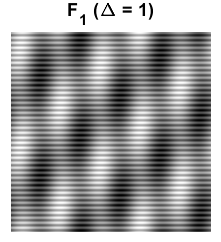
\includegraphics[scale=1]{../imgs/q1_1.png}
\end{minipage}
\vskip 0.1in

\subsection{}
The 2D FFT was used to create the Fourier representation of the image. The Amplitudes are the following:

\vskip 0.1in
\begin{minipage}{0.5\textwidth}
	\centering
	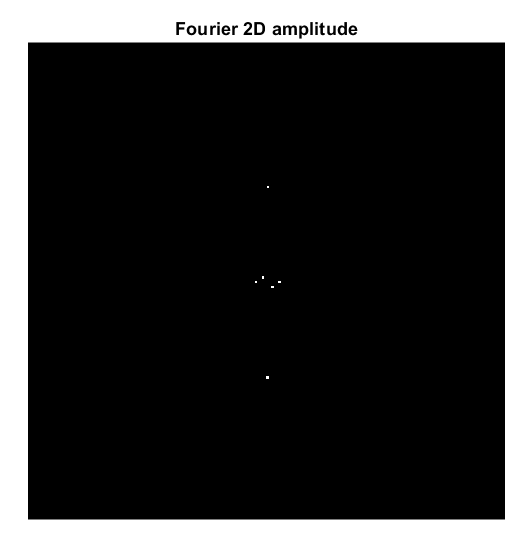
\includegraphics[scale=0.7]{../imgs/q1_2.png}
\end{minipage}
\vskip 0.1in

As expected, we can see 6 deltas, according to the 3 frequencies that are present in the image:

\begin{enumerate}
\item Two dots on the vertical line $\rightarrow$ high frequency sine: $sin(2\pi \cdot \frac{y}{5})$
\item Two dots on the horizontal line $\rightarrow$ $sin(2\pi \cdot \frac{x}{20}))$
\item Two dots on the diagonal line (smallest frequencies) $\rightarrow$ $sin(2\pi \cdot \frac{x+y}{50})$
\end{enumerate}

To understand it easier, we have colored those lines:

\vskip 0.1in
\begin{minipage}{0.5\textwidth}
\centering
	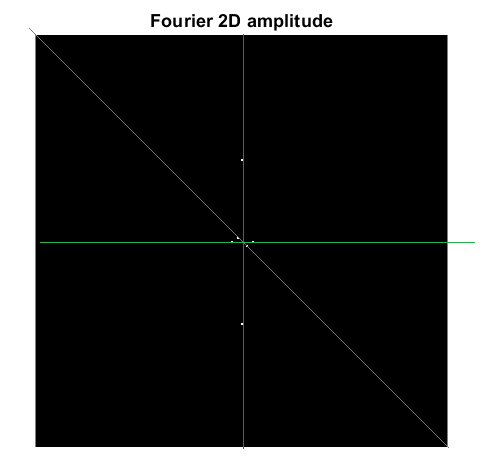
\includegraphics[scale=1]{../imgs/q1_2_colored.png}
\end{minipage}
\vskip 0.1in

The exact coordinated of the deltas are:

% Please add the following required packages to your document preamble:
% \usepackage{multirow}
\begin{table}[]
\begin{tabular}{|c|c|c|c|c|}
\hline
                            & Row & Col & Distance from center (px) & Frequency             \\ \hline
Middle point                & 101 & 101 &                           &                       \\ \hline
\multirow{2}{*}{$sin(2\pi \cdot \frac{y}{5})$} & 61  & 101 & \multirow{2}{*}{40}       & \multirow{2}{*}{0.2}  \\ \cline{2-3}
                            & 141 & 101 &                           &                       \\ \hline
\multirow{2}{*}{$sin(2\pi \cdot \frac{x}{20})$}  & 101 & 96  & \multirow{2}{*}{5}        & \multirow{2}{*}{0.05} \\ \cline{2-3}
                            & 101 & 106 &                           &                       \\ \hline
\multirow{2}{*}{$sin(2\pi \cdot \frac{x+y}{50})$}  & 99  & 99  & \multirow{2}{*}{2.82}     & \multirow{2}{*}{0.02} \\ \cline{2-3}
                            & 103 & 103 &                           &                       \\ \hline
\end{tabular}
\end{table}

We can see that the distance from center fits the frequency. For example, the highest distance from center for $y$ is 100 pixels, which corresponds to the highest frequency that the image can display with sample size of 1: $f = 0.5$. Thus, for frequency of 0.2, we obtain distance $100\cdot \frac{0.2}{0.5} = 40$. 


\subsection{}
The image was not sampled with a sampling size ($\Delta$) of 9 $(S+1) = 8+1 = 9$. This sampleing size corresponds to a frequency of $\frac{1}{9} = 0.11111...$. After performing the same procedure, the Fourier transform was found to give the following amplitures map:

\vskip 0.1in
\begin{minipage}{0.8\textwidth}
\centering
	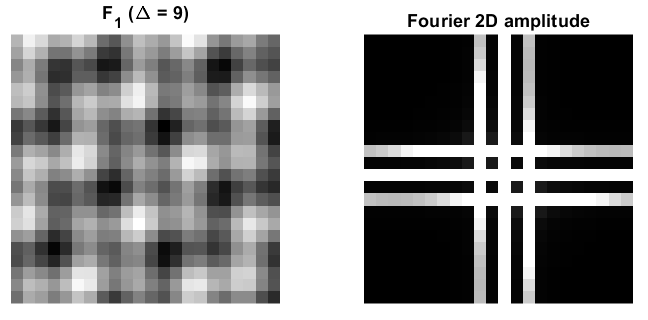
\includegraphics[scale=0.7]{../imgs/q1_3.png}
\end{minipage}
\vskip 0.1in

We can clearly see the aliasing here. But the aliasing only occurs on the first 1 terms in $F_{1}$. To avoid aliasing, we are required to sample at least at the frequency which is twice higher than the frequency of the signal, e.g. 0.4. But we sample at a much lower rate - 0.1111... The existance of this diversity of frequency (lines) shows that we sample at the frequency which does not align with the given sine frequency, not matter how we multiply both. For example, if we sample at the Sample Size of 4, which corresponds to the frequency of 0.25, we alias the $sin(2\pi \cdot \frac{y}{5})$ function another sine wave function of lower frequency which has consistent common intersections with the original sine wave. We can see this on the following FFT transform. Notice how the dots on the vertical lines came closer to the center:
\vskip 0.1in
\begin{minipage}{0.8\textwidth}
\centering
	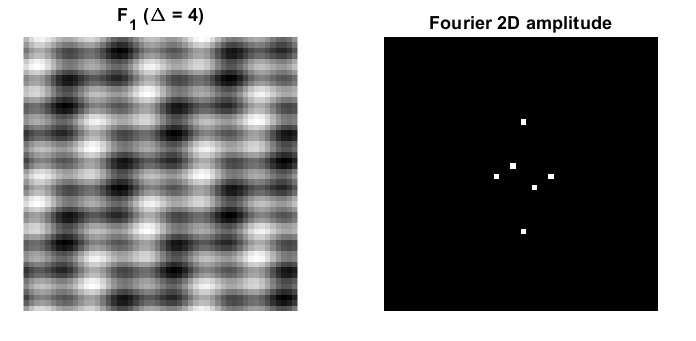
\includegraphics[scale=0.8]{../imgs/q1_3_1.png}
\end{minipage}
\vskip 0.1in

Or we can choose a sample rate which will alias this sine wave ($sin(2\pi \cdot \frac{y}{5})$) function with a constant value! We have to choose a sample size, which corresponds exactly to the period of the sine wave, which is 10 pixels. This way we always fall onto '0' value of this function:

\vskip 0.1in
\begin{minipage}{0.8\textwidth}
\centering
	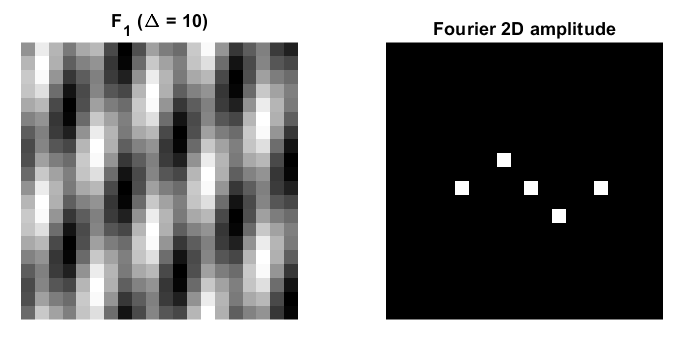
\includegraphics[scale=0.8]{../imgs/q1_3_2.png}
\end{minipage}
\vskip 0.1in




%\begin{equation}
%\end{equation}



\subsection{}
A real image was taken, from the internet. The image contains various elements, windows at buildings, and other things which have high frequencies. Image was resized to 400x400 px. Plotting the image and its 2D FFT amplitudes gives:

\vskip 0.1in
\begin{minipage}{1\textwidth}
\centering
	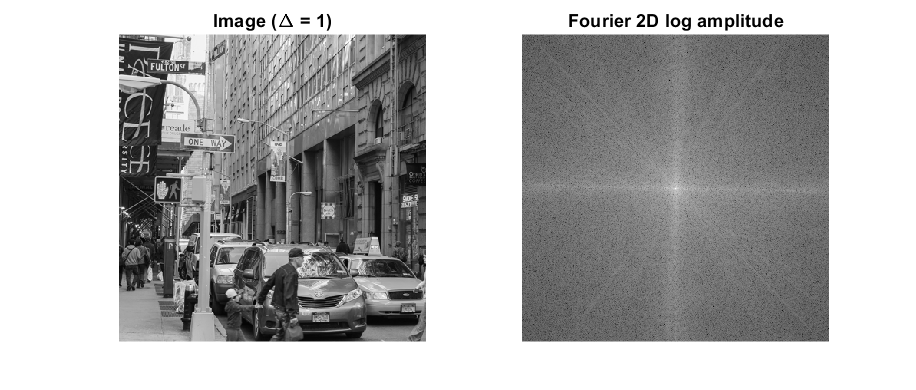
\includegraphics[scale=0.7]{../imgs/q1_5.png}
\end{minipage}
\vskip 0.1in

\subsection{}
The sampling with the a sampling size of 4 was performed. The resulting image is of size 100x100 px. Plotting the image and its 2D FFT log amplitude. To answer the question, we plot the images together with the original image, for convenience.


\vskip 0.1in
\begin{minipage}{1\textwidth}
\centering
	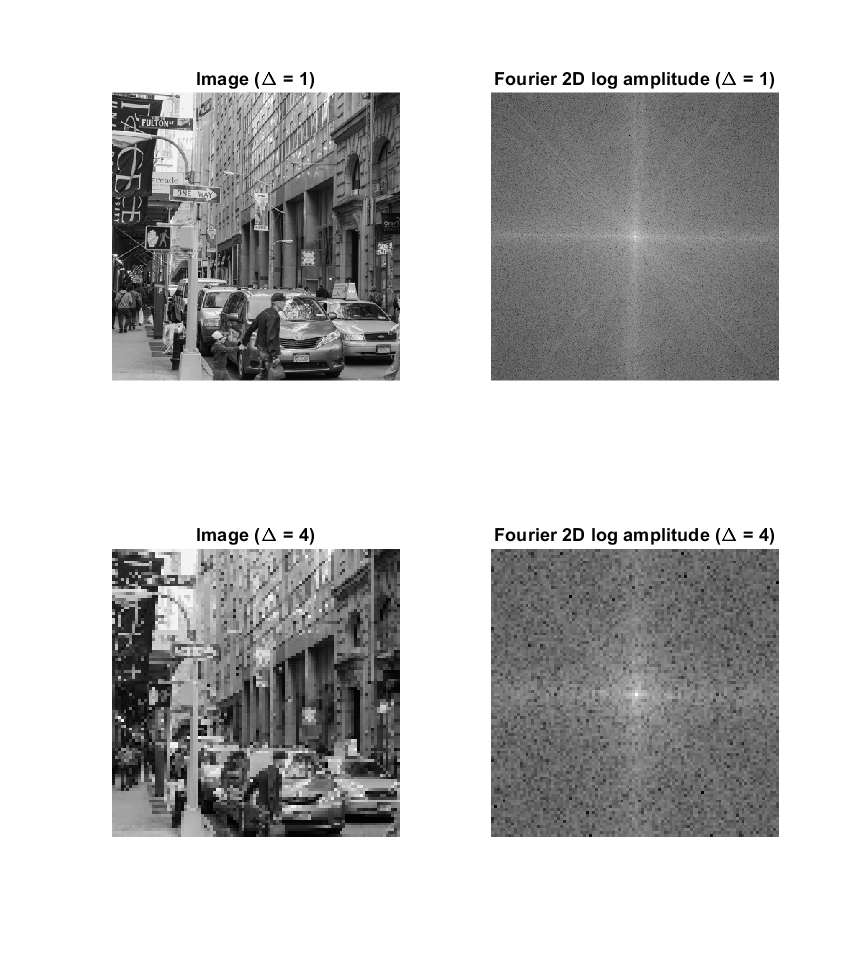
\includegraphics[scale=0.7]{../imgs/q1_6.png}
\end{minipage}
\vskip 0.1in

Differences:
\begin{enumerate}
\item In spatial domain: we can see that the details that were small are not visible anymore, disappeared, because the sampling rate was too small to preserve them, and they got aliased with frequencies, which are smaller than Nyquist frequencies. Thus, those details are not visible anymore.
\item In frequency domain: We can see that the high frequencies got less intense, and most of them disappeared. We can see a shift towards the center of the frequencies plot, where the frequencies are lower. It happened because some high frequencies got aliased by the low frequencies, so their intensity rised.
\end{enumerate}

\subsection{}
In this subsection we first apply the Gaussian filter on the original image, and only then subsample. The results are the following:

\vskip 0.1in
\begin{minipage}{1\textwidth}
\centering
	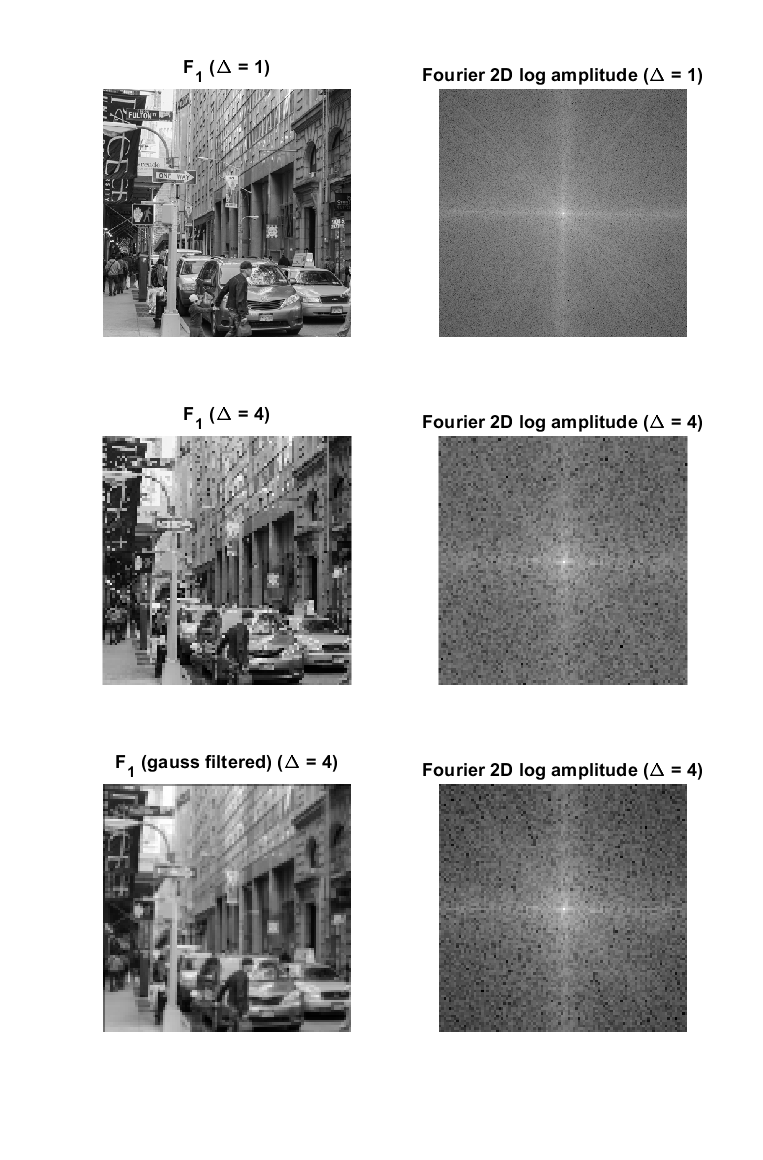
\includegraphics[scale=0.7]{../imgs/q1_7.png}
\end{minipage}
\vskip 0.1in

We can observe that here, the high frequencies were better preverved! This is indeed one of the methods to reduce the aliasing effect. Because we have applied the Gaussian filter, which is the LPF, the high frequencies were reduced, thus not creating the aliasing effect. 




\newpage
\section{Question 2}

\subsection{}
video was played.

\subsection{}
One (1) cycle is being completed within 20 frames. Thus, the cycle time is 20 frames/cycle. The video is being played in 20 [frames/sec], thus, the cycle frequency is 1 [cycle/sec]. The following image shows 1 cycle:

\vskip 0.1in
\begin{minipage}{1\textwidth}
\centering
	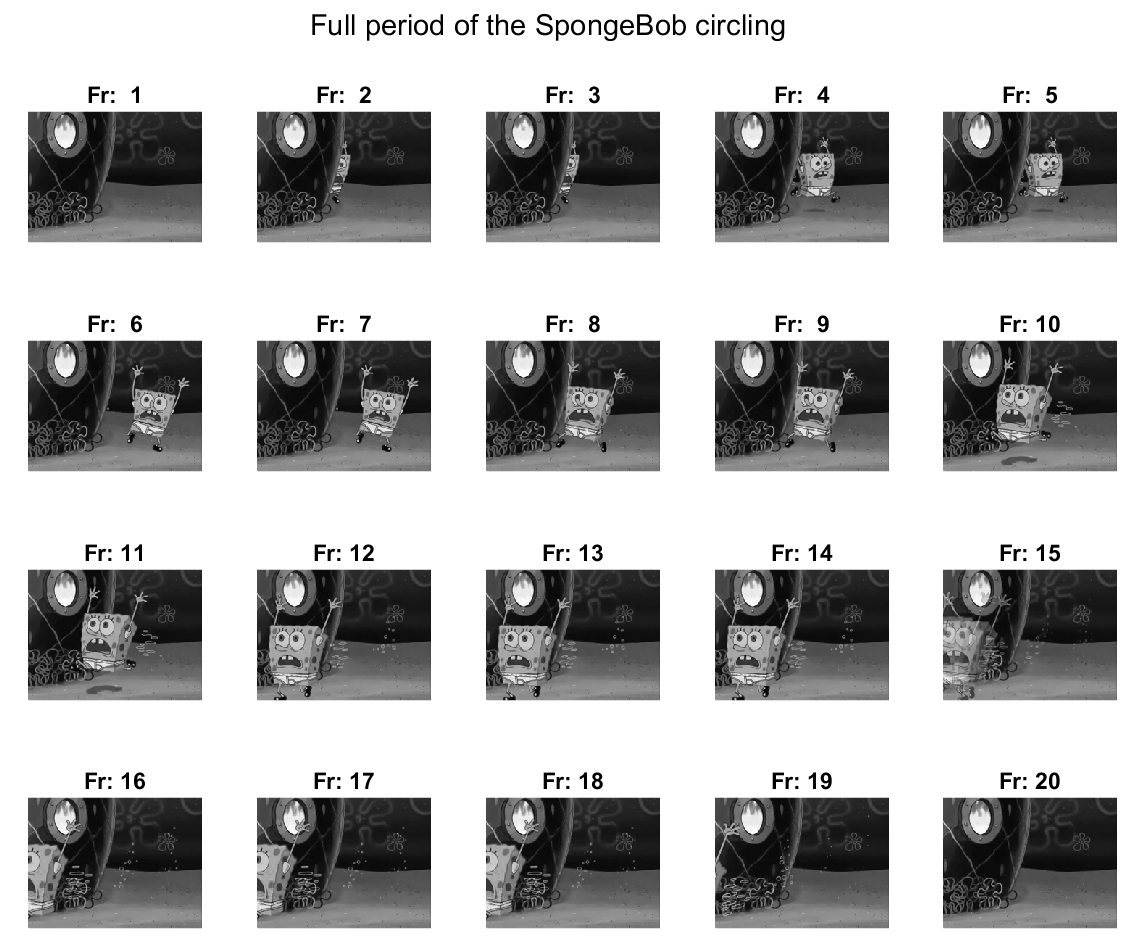
\includegraphics[scale=0.9]{../imgs/imgs_q2/sponge_period.png}
\end{minipage}
\vskip 0.1in
\subsection{}
The Nyquist frequency to sample the video is twice the maximum frequency of the spin frequency. Thus:
$$f_{nyquist} = 2 [spin/sec] = 40 [FPS]$$

\subsection{}
In order to see the video backwards, we need to sample it at a frequency smaller than the Nyquist frequency. The sampling period is 0.5 frames for Nyquist frequency. If we take, for example, sampling period of 15, we are way below the Nyquist frequency and obtain the backward-moving SpongeBob:


\vskip 0.1in
\begin{minipage}{1\textwidth}
\centering
	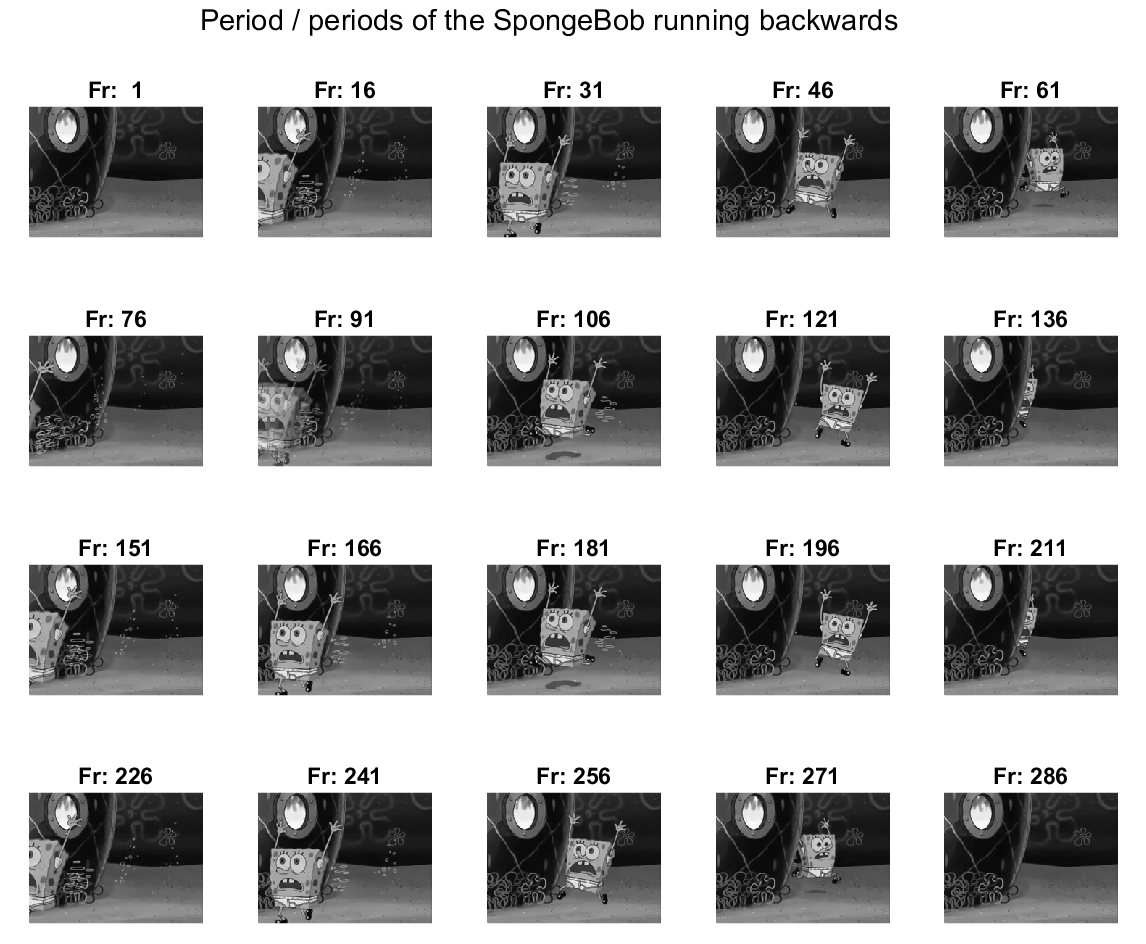
\includegraphics[scale=0.9]{../imgs/imgs_q2/sponge_period_backwards.png}
\end{minipage}
\vskip 0.1in

















\newpage
\section{Question 3}

\subsection{}
The function was implemented in MATLAB

\subsection{}
The entropy for the 'heisenberg.jpg' image was calculated to be $7.011$. 

\subsection{}
The function was implemented in MATLAB

\subsection{}
The huffman code was created. The resulting data rate is 7.034 [bits/symbol] (which is smaller than the usual 8 [bits/symbol/ required for the symbol of range 0-255). We can notice that this value is a bit larger than the entropy, but is very close to it. The compression ratio is being calculated: $$CR = \frac{log2(256)}{7.034} = 1.137$$

\subsection{}
The image was decoded using the mentioned decoding function. The MSE calculated is 0. This is because this compression method is lossless, and no data is being lost during the process. (unlike Quantization, for example).

\subsection{}
Differences encoding:
\subsubsection{}
Was done.
\subsubsection{}
The differences vector was calculated, and reshaped back to original size. The histograms for both of the differences images are the following:
\vskip 0.1in
\begin{minipage}{1\textwidth}
\centering
	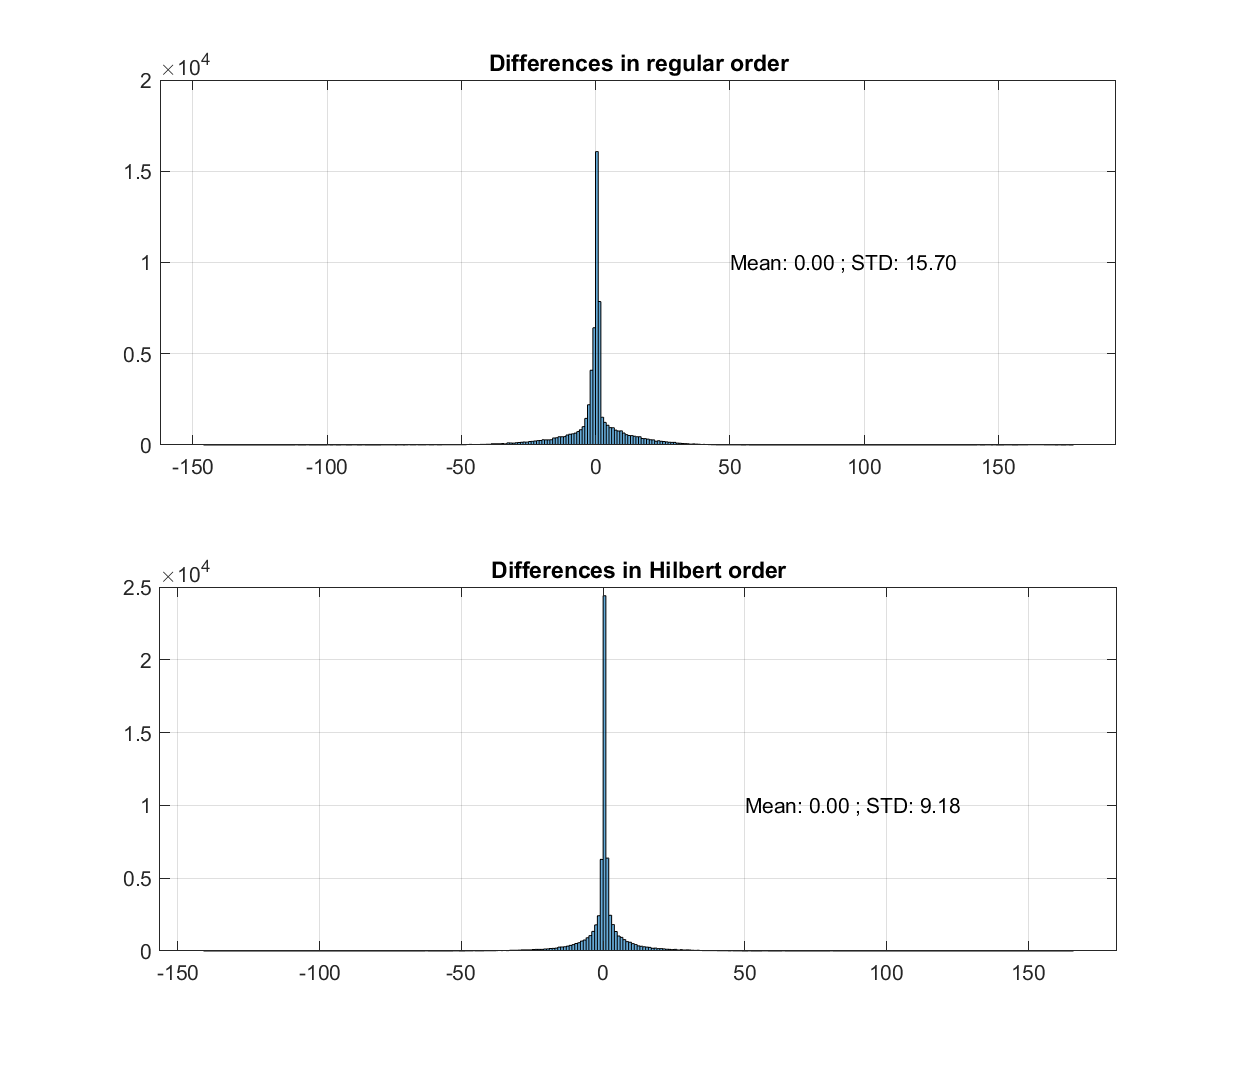
\includegraphics[scale=0.9]{../imgs/imgs_q3/q3_histograms_comp.png}
\end{minipage}
\vskip 0.1in

We have as well printed the STD and the Mean values to emphasize the difference. We can clearly see that the differences between pixels in the Hilbert's ordering method are smaller. This happens, because its order assumes that the similar regions in the image stay together, and do not tend to span in horizontal or vertical direction. Thus, we obtain, that in overall, the differences span on a smaller scale.


\subsubsection{}
The Huffman code was built for both differences images. We already expect that the data rate for the image with smaller values span (and smaller Variance) will be larger, and will have greater compression rate. Let's verify this.

\begin{enumerate}
\item For the regular ordered image:
	\begin{enumerate}
	\item $Data rate = 4.779 [bits/symbol]$
	\item $CR = 1.674$
	\end{enumerate}
\item For the Hilbert ordered image:
	\begin{enumerate}
	\item $Data rate = 4.105 [bits/symbol]$
	\item $CR = 1.949$
	\end{enumerate}
\end{enumerate}

We can clearly see that the CR for the Hilbert ordered image is higher. And that the differences encoding gives us much better CR than the encoding of the original pixels values.













\newpage
\section{Question 4}

\subsubsection{}
The function was created. See MATLAB code.

\subsubsection{}
The quantization was performed on the selected image, and the following results have been obtained. The graphs are displayed in all cased in the following order: (1) The quantized image (2) the distortion levels (3) the relative improvement

For the 6 levels quantization:

\vskip 0.1in
\begin{minipage}{1\textwidth}
\centering
	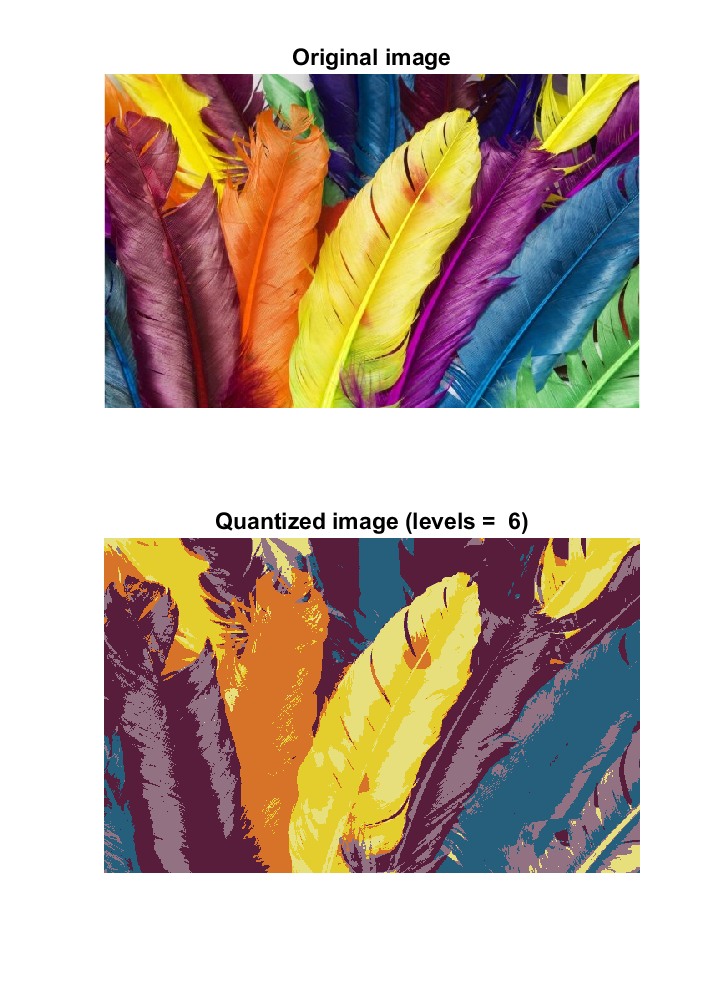
\includegraphics[scale=0.9]{../imgs/imgs_q4/q4_quantized_levels_6_init_1.png}
\end{minipage}
\vskip 0.1in

\vskip 0.1in
\begin{minipage}{1\textwidth}
\centering
	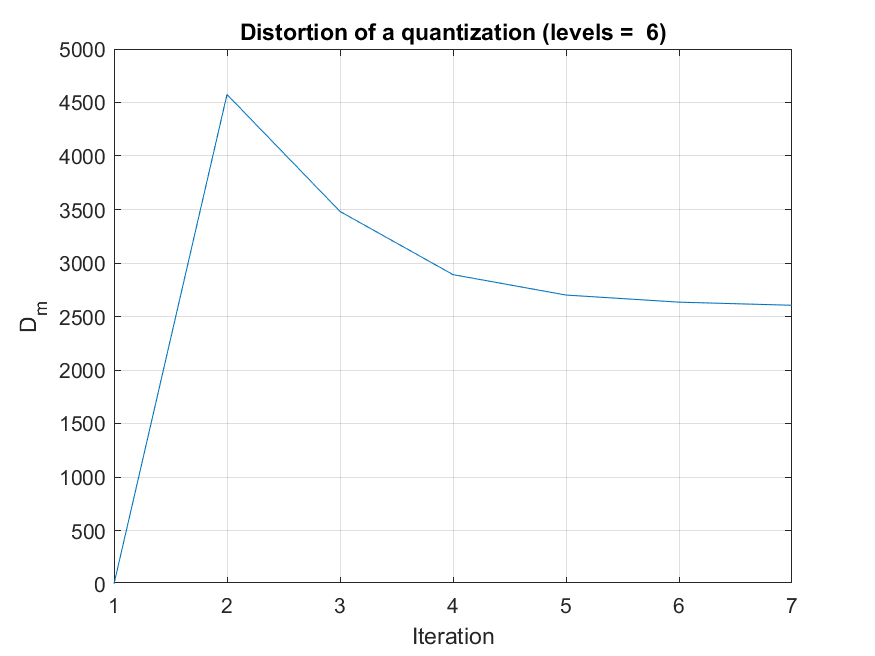
\includegraphics[scale=0.9]{../imgs/imgs_q4/q4_distortion_levels_6_init_1.png}
\end{minipage}
\vskip 0.1in

\vskip 0.1in
\begin{minipage}{1\textwidth}
\centering
	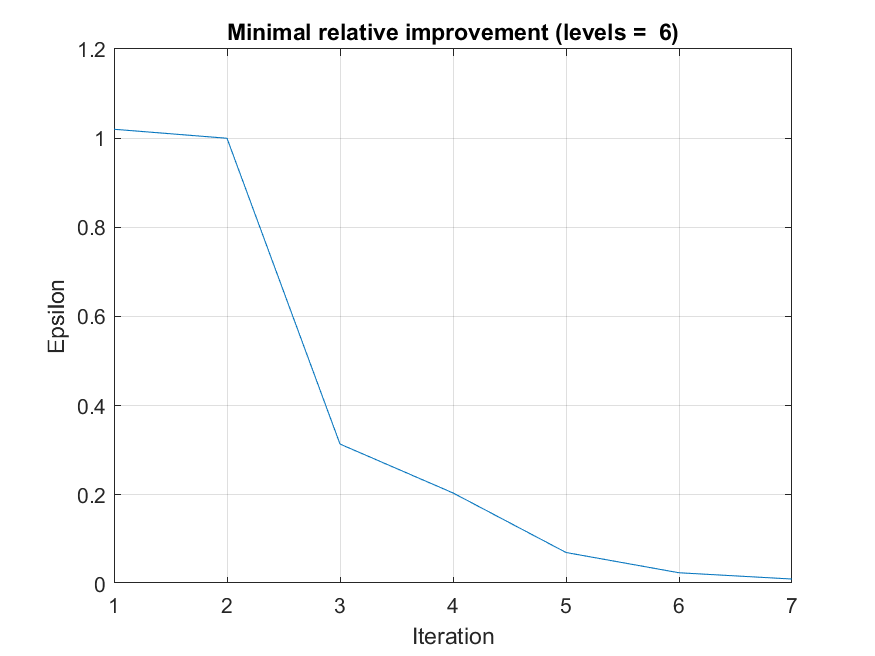
\includegraphics[scale=0.9]{../imgs/imgs_q4/q4_epsilon_levels_6_init_1.png}
\end{minipage}
\vskip 0.1in


For the 15 levels quantization:

\vskip 0.1in
\begin{minipage}{1\textwidth}
\centering
	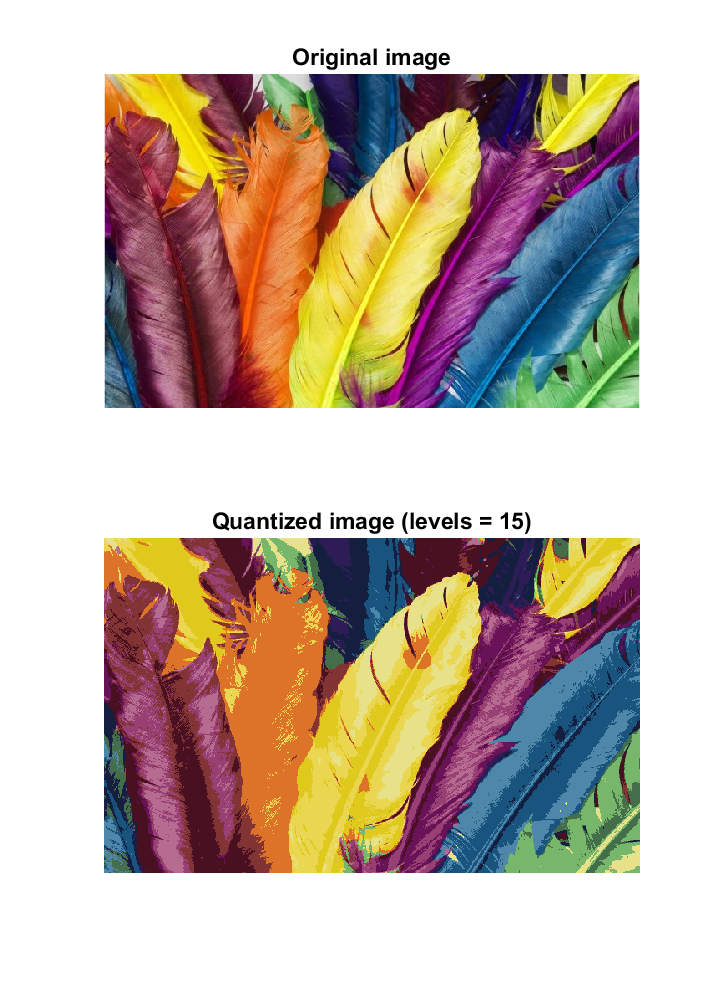
\includegraphics[scale=0.9]{../imgs/imgs_q4/q4_quantized_levels_15_init_1.png}
\end{minipage}
\vskip 0.1in

\vskip 0.1in
\begin{minipage}{1\textwidth}
\centering
	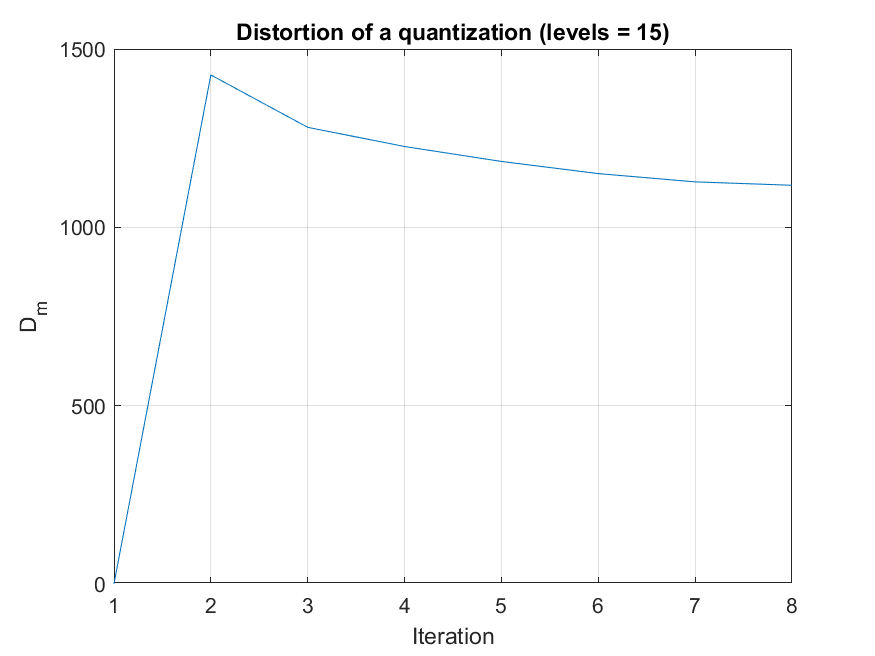
\includegraphics[scale=0.9]{../imgs/imgs_q4/q4_distortion_levels_15_init_1.png}
\end{minipage}
\vskip 0.1in

\vskip 0.1in
\begin{minipage}{1\textwidth}
\centering
	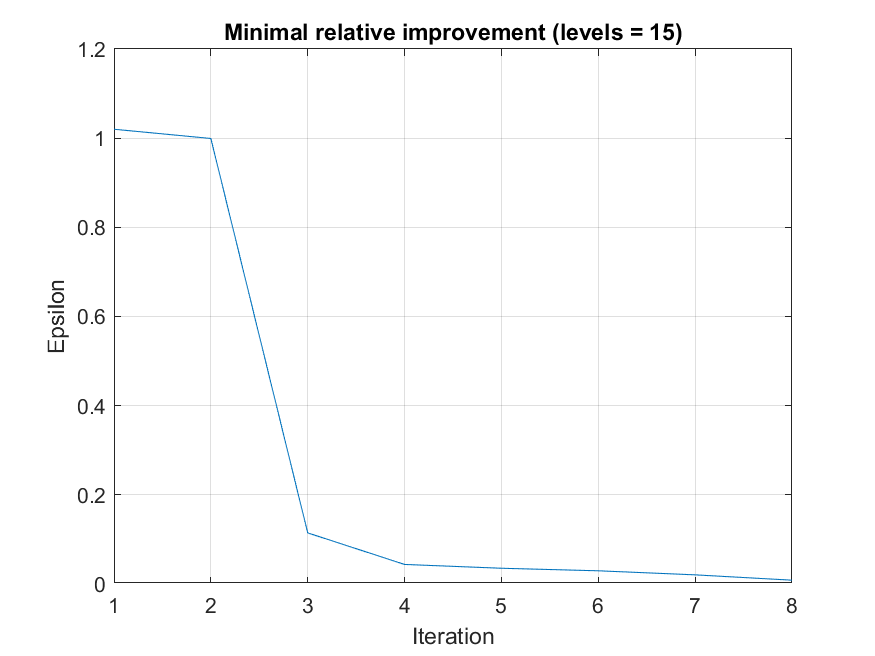
\includegraphics[scale=0.9]{../imgs/imgs_q4/q4_epsilon_levels_15_init_1.png}
\end{minipage}
\vskip 0.1in


\subsubsection{}
Indeed, if we re-run the algorithm, the results will be different each time. This happens because we instantiate the algorithm randomly, picking random pixels and taking their representations as representative levels. We may find numerous local minimas where the algorithm will be unable to find a more optimal solution.  The algorithm stops when the improvement is very little, meaning it has reached its local minimum point. Numerous local minimums can give numerous representations, and their distortion is not the same.


\subsubsection{}
We have extended the algorithm to accept also the parameter of initialization. This time, for the 9 levels, the results are the following:


\vskip 0.1in
\begin{minipage}{1\textwidth}
\centering
	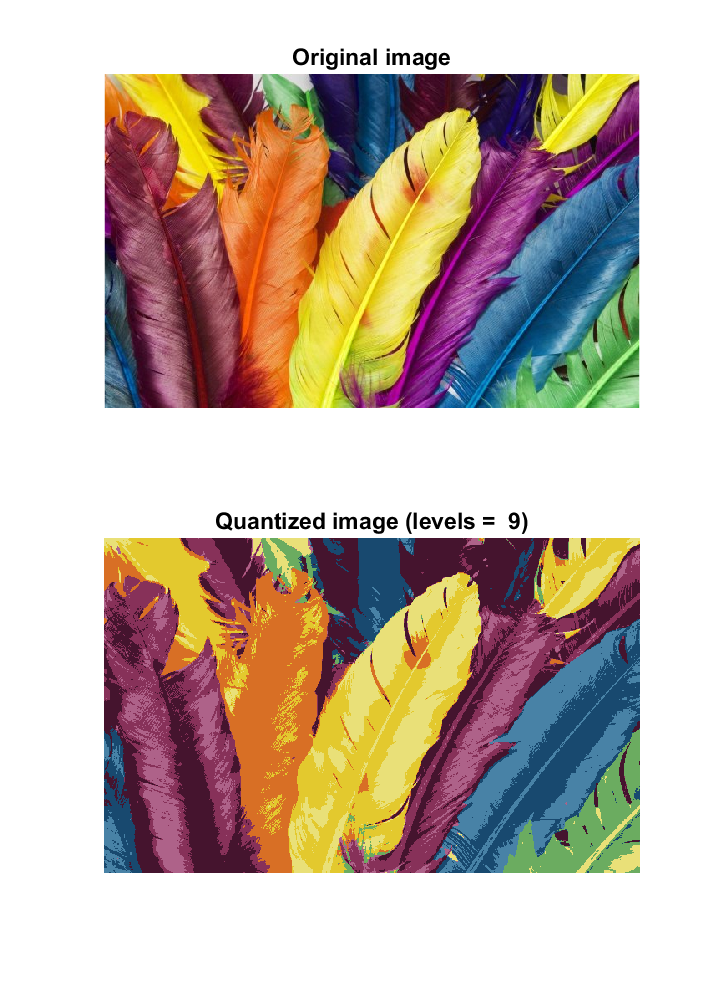
\includegraphics[scale=0.9]{../imgs/imgs_q4/q4_quantized_levels_9_init_2.png}
\end{minipage}
\vskip 0.1in

\vskip 0.1in
\begin{minipage}{1\textwidth}
\centering
	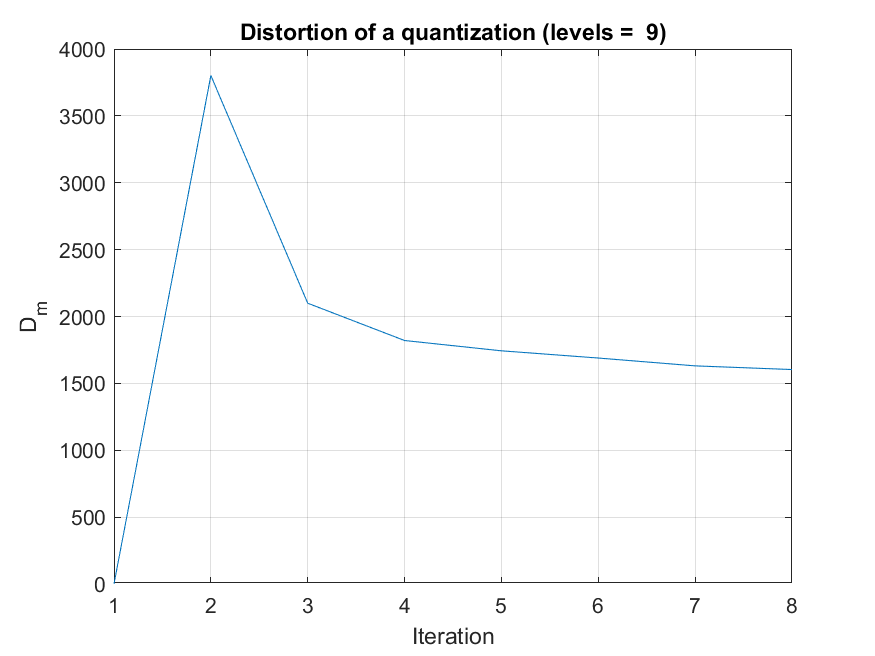
\includegraphics[scale=0.9]{../imgs/imgs_q4/q4_distortion_levels_9_init_2.png}
\end{minipage}
\vskip 0.1in

\vskip 0.1in
\begin{minipage}{1\textwidth}
\centering
	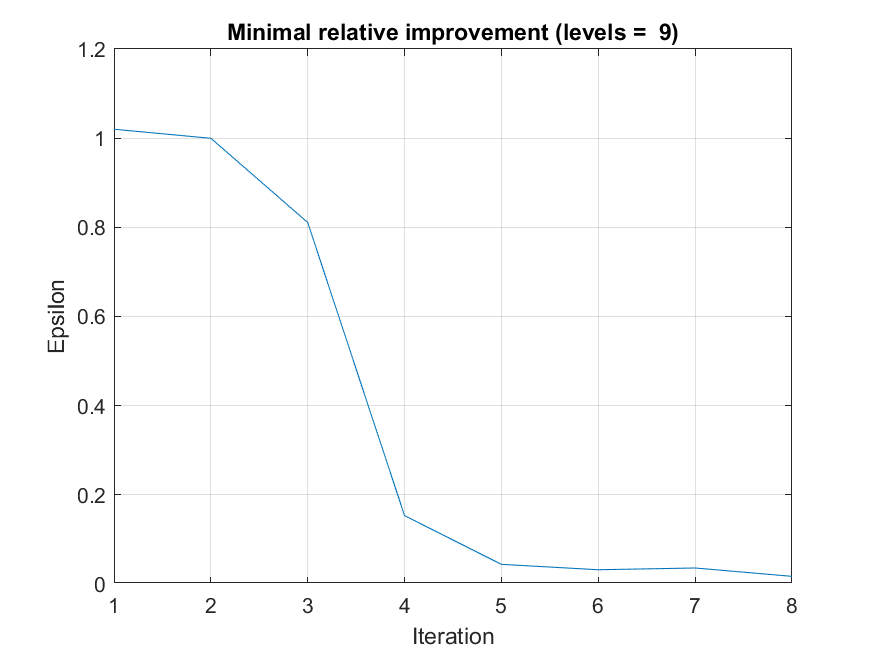
\includegraphics[scale=0.9]{../imgs/imgs_q4/q4_epsilon_levels_9_init_2.png}
\end{minipage}
\vskip 0.1in

\subsubsection{}
In this case, the colors were not picked randomly. We have used the prior information, and assumed that the colors will be spanned through the variety of spectrum. Several conclusions may be drawn:

\begin{enumerate}
\item By having a fixed initial representation, each new run of an algorithm gives the same result.
\item We did not observe improvement in iterations number. By logically, yes, the iterations number should be smaller. Perhaps, if we run the algorithm numerous times, we can observe it.
\item Comparing to the 15-levels, random initialization, the distortion for 9-level fixed initialization is larger. Because, still, the levels amout is a major factor in the distorion.
\item When the algorithm was re-run on 9 levels random initialization, the distortion obtained was larger. Which proves that using a prior information on a color spectrum helps to deliver the best quantization initial parameters
\end{enumerate}










\newpage
\section{Question 5}

\subsubsection{}
The function was created. See MATLAB code.

\subsubsection{}
The Gaussian and Laplasian pyramids for both of the images were created and the results are the following:

The Gaussian pyramid for apple:
\vskip 0.1in
\begin{minipage}{1\textwidth}
\centering
	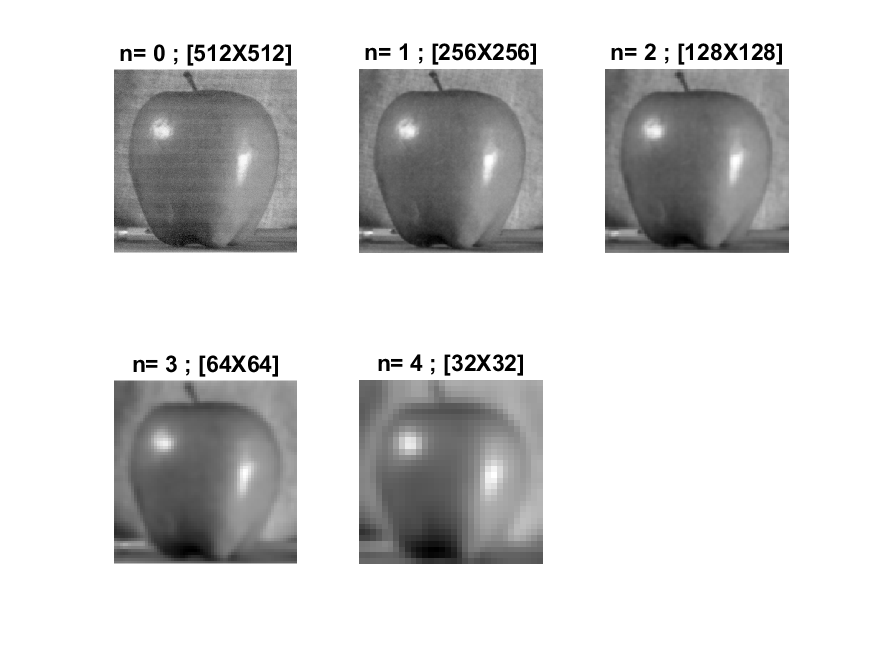
\includegraphics[scale=0.9]{../imgs/imgs_q5/q5_apple_gaus.png}
\end{minipage}
\vskip 0.1in

The Laplasian pyramid for apple:
\vskip 0.1in
\begin{minipage}{1\textwidth}
\centering
	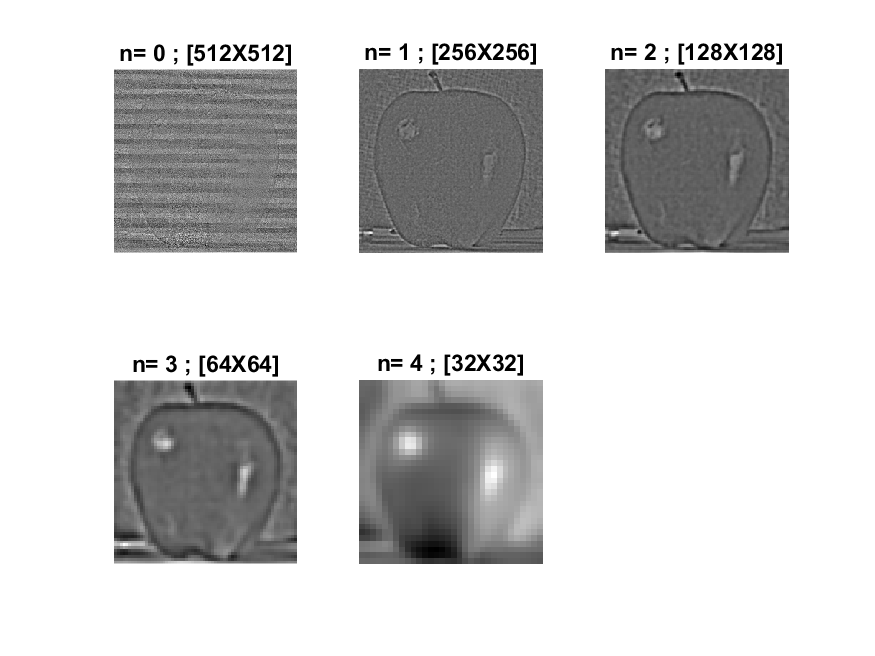
\includegraphics[scale=0.9]{../imgs/imgs_q5/q5_apple_lap.png}
\end{minipage}
\vskip 0.1in

The Gaussian pyramid for orange:
\vskip 0.1in
\begin{minipage}{1\textwidth}
\centering
	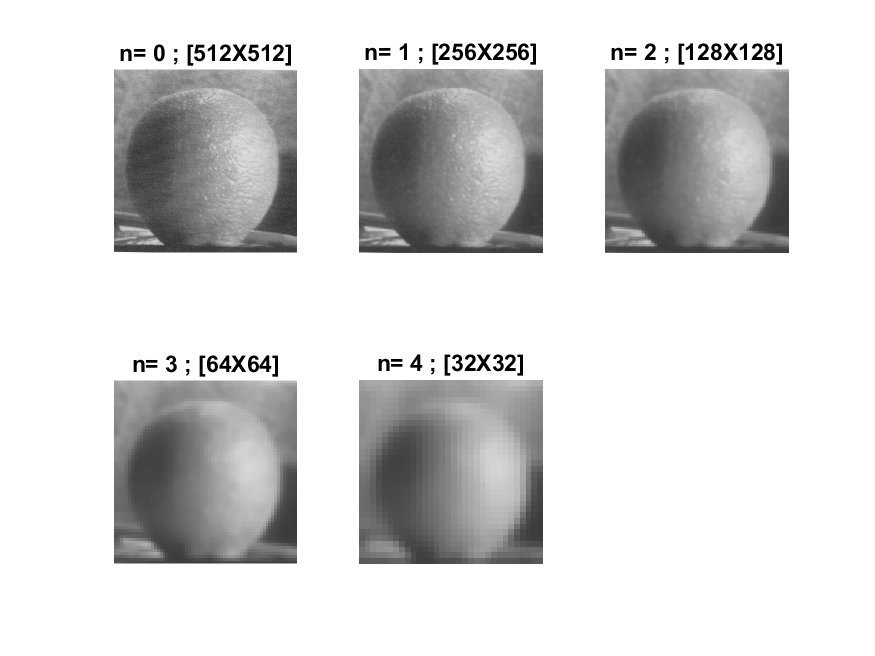
\includegraphics[scale=0.9]{../imgs/imgs_q5/q5_orange_gaus.png}
\end{minipage}
\vskip 0.1in

The Laplasian pyramid for orange:
\vskip 0.1in
\begin{minipage}{1\textwidth}
\centering
	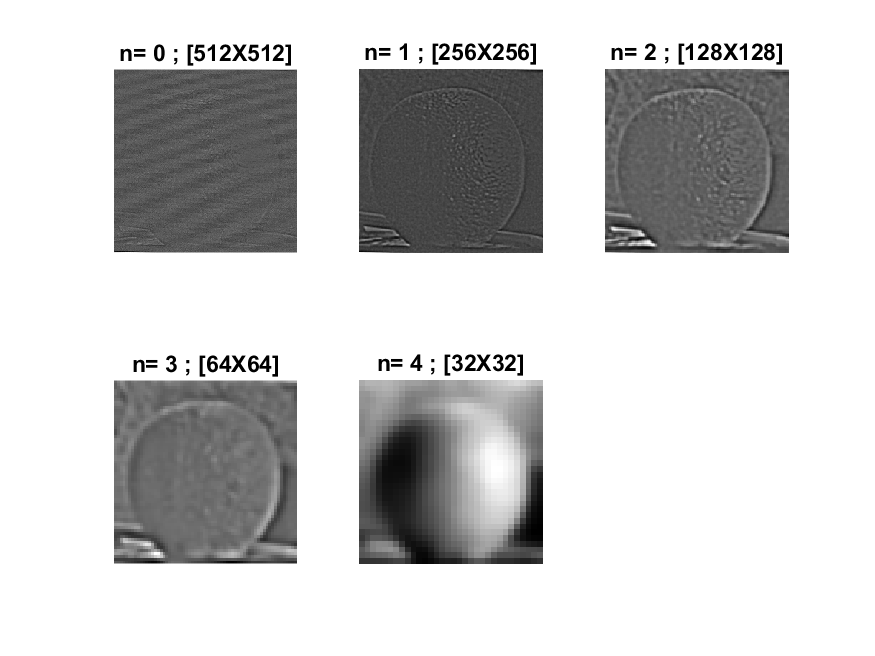
\includegraphics[scale=0.9]{../imgs/imgs_q5/q5_orange_lap.png}
\end{minipage}
\vskip 0.1in


\subsubsection{}
The function was created. See MATLAB code.

\subsubsection{}
The apple and orange images were reconstructed. We also show the difference between the original image and the reconstructed image to verify there are no differences:

Apple reconstructed:
\vskip 0.1in
\begin{minipage}{1\textwidth}
\centering
	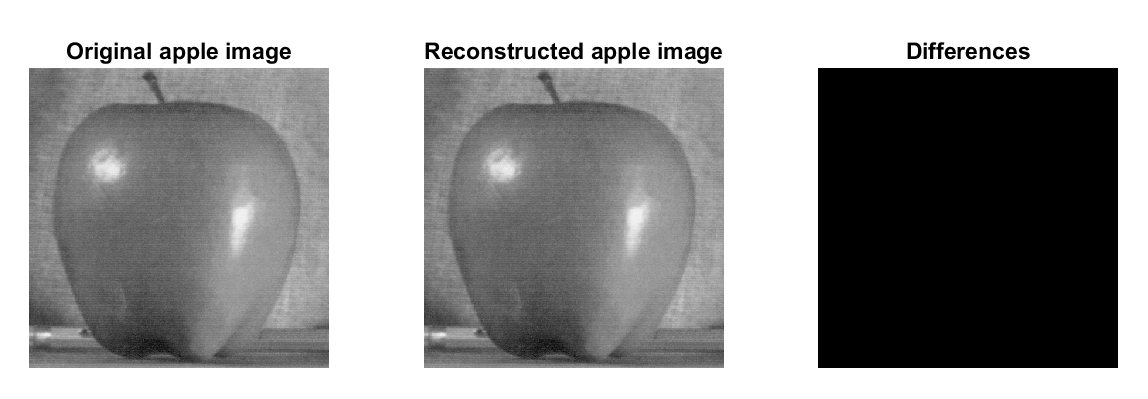
\includegraphics[scale=0.9]{../imgs/imgs_q5/q5_apple_reconstructed.png}
\end{minipage}
\vskip 0.1in


Orange reconstructed:
\vskip 0.1in
\begin{minipage}{1\textwidth}
\centering
	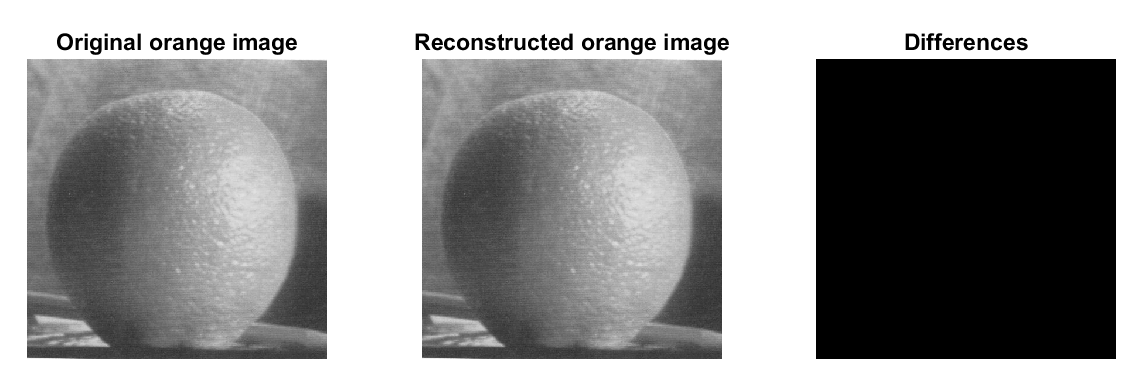
\includegraphics[scale=0.9]{../imgs/imgs_q5/q5_orange_reconstructed.png}
\end{minipage}
\vskip 0.1in


\subsubsection{}
Image mosaic implementation. The function was created, the number of common pixels is the parameter which user can input. Following the instructions, we set this parameter to be '2'. The results are the following:


\vskip 0.1in
\begin{minipage}{1\textwidth}
\centering
	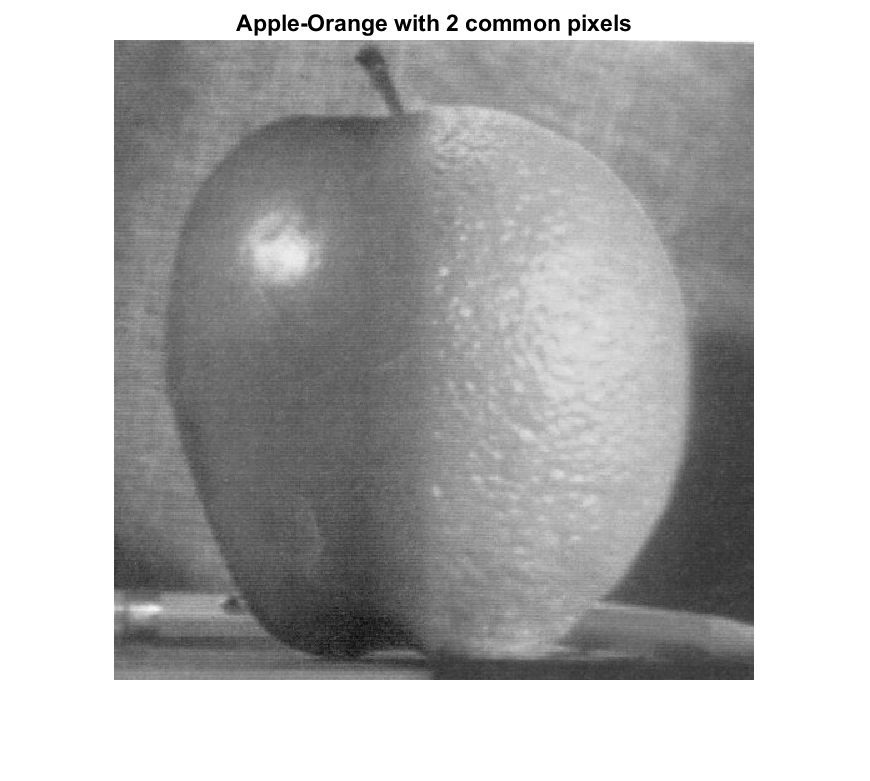
\includegraphics[scale=0.9]{../imgs/imgs_q5/q5_apple_orange_lapl_1.png}
\end{minipage}
\vskip 0.1in

The Laplasian pyramid of the mosaic image:

\vskip 0.1in
\begin{minipage}{1\textwidth}
\centering
	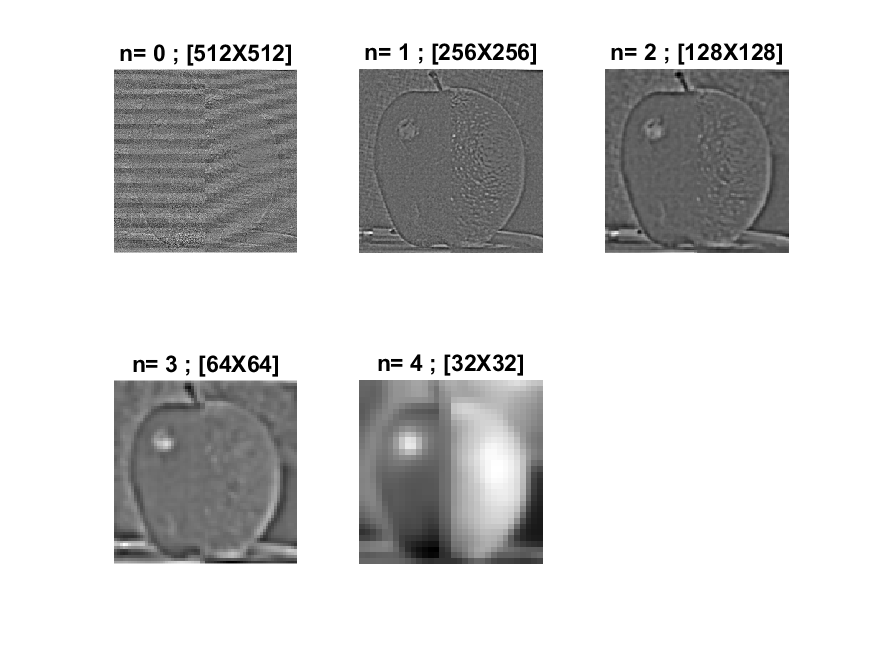
\includegraphics[scale=0.9]{../imgs/imgs_q5/q5_apple_orange_lapl.png}
\end{minipage}
\vskip 0.1in


\subsubsection{}
By doing a simple stitch, by simply putting images together on different Laplasian pyramid levels, we obtain:

\vskip 0.1in
\begin{minipage}{1\textwidth}
\centering
	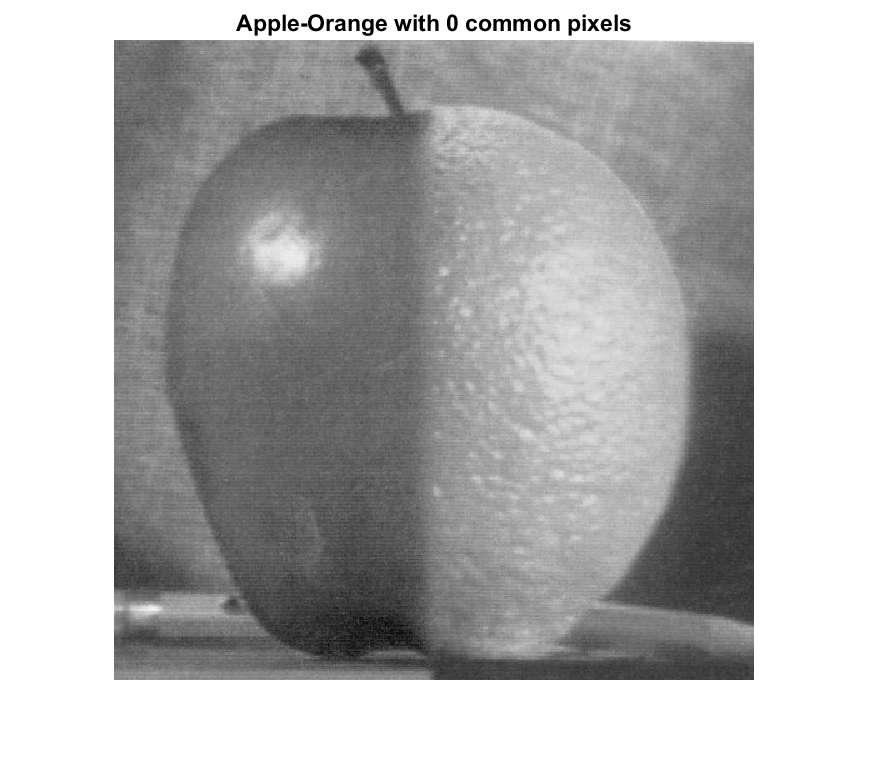
\includegraphics[scale=0.9]{../imgs/imgs_q5/q5_apple_orange_lapl_2.png}
\end{minipage}
\vskip 0.1in

Comparing this to the first stitching, we can see the differences:
\vskip 0.1in
\begin{minipage}{1\textwidth}
\centering
	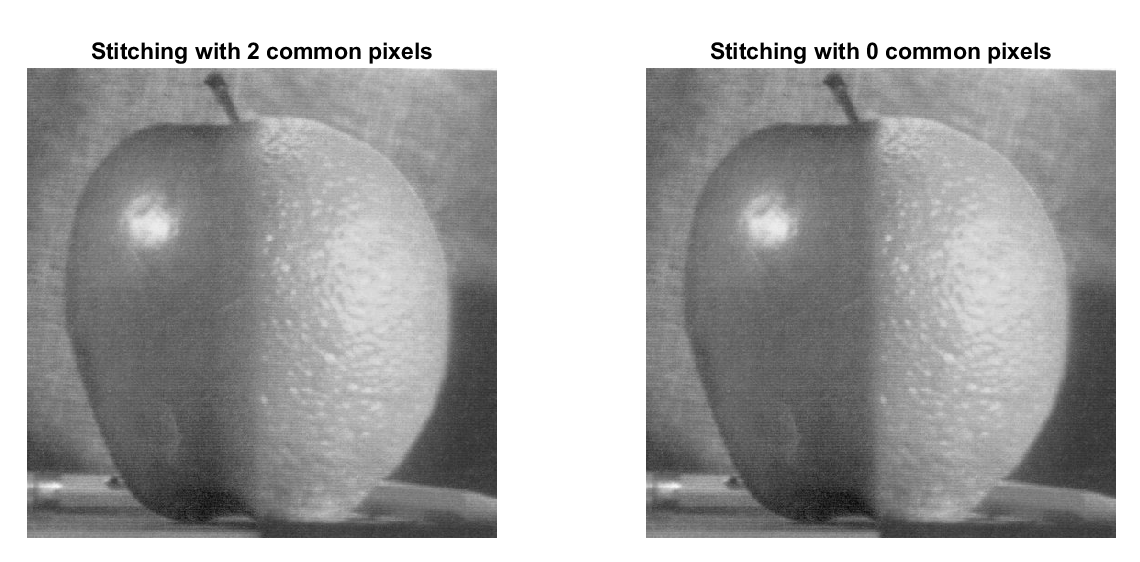
\includegraphics[scale=0.9]{../imgs/imgs_q5/q5_apple_orange_comp.png}
\end{minipage}
\vskip 0.1in

We can indeed observe that the "transition" stage between the images becomes more "smooth" as the number of "common pixels" increases. This can be logically explained, since we share the pixels information further "deeper" into the images. But also with a simple method of putting images side-by-side does achieve transition. This happens because the 'expand' function, which is used in the reconstruction phase from the Laplasian pyramid, uses the information of the neighboring pixels in its process.







\end{document}



















